
% modeling Dominion in Hakaru, and what kinds of questions are interesting
% to ask the model
\section{Dominion} \label{sec:dom}

Dominion is a game we are familiar with. This game is known as a turn-based
deckbuilding game, where a player \emph{builds} a good deck by choosing what
cards to buy on their turn. The probabilistic component of deckbuilding games
arises from shuffling decks of cards at certain points in the game. In particular
in Dominion the cards a player plays can affect both when cards get shuffled
and the composition of the deck being shuffled. As a result, game-play heuristics
for Dominion are inherently intertwined with the probabilistic game state.

\subsection{Game State}

\subsection{Heuristics} \label{sec:dom:heuristics}
We

% -----------------------------------------------------------------------------
% Theory of the greedy-vs-greedy experiment
\subsection{Greedy Theory}
A simple query one might wish to ask of the greedy heuristic is:

\begin{quote} \label{quote:dominion-query}
Given that we buy card $X$ with probability $p_0$ and card $Y$ with
probability $(1 - p_0)$, what is the distribution over the length of
the game?
\end{quote}

In this query, we have model parameters comprising:

\begin{itemize}
\item $X$  \hsk{:: Card}
\item $Y$  \hsk{:: Card}
\item $p_0$ \hsk{:: Probability}
\end{itemize}

We also have implicit hyper-parameters comprising (see Appendix
\ref{appendix:runtime-cards} for an overview of the Haskell
implementation):

\begin{itemize}
\item \hsk{kingdomCards :: [Card]}
\item \hsk{turnRules    :: [GameParameters]}
\end{itemize}



One observe-query inference question to ask the model then is:

\begin{equation} \label{q:inference}

\end{equation}

% -----------------------------------------------------------------------------
% Results figures:
\subsection{Greedy Results \& Analysis} \label{sec:dom:greedy-results}
We now present results for the greedy heuristic, as described in
Section \ref{sec:dom:heuristics}. Before answering the inference
question (Question \ref{q:inference}), we first take unconditioned
samples from the greedy-vs-greedy model to determine characteristic
game lengths. The result of this sampling is realized as a
gaussian-like distribution of Figure \ref{fig:turn-dist}. Sampling
the model with other values of the \hsk{VILLAGE} - \hsk{CHANCELLOR}
buy ratio $p_0$ shows that $p_0$ is inversely related to the mean
of the gaussian $\mu_{t}$.

From this information we infer that the \hsk{VILLAGE} card has
a greater impact on how quickly the game ends. This is interesting
to a player of Dominion attempting to come up with a ranking of
cards. Performing an automated analysis on every possible pair
of cards using this sampling technique, one could:

\begin{itemize}
\item Design a good greedy buy heuristics
\item Determine the balance of the hyper-parameter corresponding
      to which cards are being used in the game.
\end{itemize}

The \hsk{VILLAGE} having a greater impact on the game ending is
also in line with the personal belief of the author that a
\hsk{VILLAGE} is, in general, more useful than a \hsk{CHANCELLOR}.
However, what the gaussian form of Figure \ref{fig:turn-dist}
does not tell us is the characteristic distribution of values of
$p_0$ for a given game length. This is what the inference Question
#\ref{q:inference} is trying to give us insight into.

%While this is
%interesting and is in line with the personal belief of the author
%that a \hsk{VILLAGE} is generally more useful than a
%\hsk{CHANCELLOR}, it does not say anything about the characteristic
%value of $p_0$ for a given game length.

%TODO:
%figure: one column showing the un-normalized (frequency) plots of
%the rejection sampling, second column showing the normalized
%(probability density) 
%OR: one column of 3 plots, with the left-hand axis corresponding to
%frequency and the right-hand y-axis corresponding to probability.
%plot the distributions / barcharts on the same graph in different
%colors / with some alpha value.

In Figure \ref{fig:rejection-sampling} we see the characteristic
form of the turn-conditioned distribution over the
\hsk{VILLAGE} - \hsk{CHANCELLOR} buy ratio ($p_0$). At first glance
these distributions appear to be linear in $p_0$. In terms of our
parameters we have the equation:

\begin{equation} \label{eqn:linear-distribution}
P(p_0 | t_e = t_e') = m(p_0, X, Y) * p_0 + b(p_0, X, Y)
\end{equation}

In this equation we now have a name for the observed random variable
`game length' ($t_e$). We also have $t_e'$ a specific value for $t_e$.
Finally the latent random variables $m$ and $b$ together comprise a
characteristic description of the conditional distribution. The
key to this equation is that $m$ and $b$ are variables which cannot
be directly sampled / observed and have a probabilistic causal affect
on the observed variable $p_0$.
Since we have no feasible means for determining the closed analytical
forms of $m$ and $b$ we have relied on the Markov Chain Monte-Carlo (MCMC)
methods as described earlier in Section \ref{sec:mcmc}.

% - the slope $m$ is a relative measure of the balance between cards
%   $X$ and $Y$, namely balance can be interpreted as proportional
%   to $1 / abs(m). A slope of exactly $m = 0$ means the cards $X$
%   and $Y$ are perfectly balanced
% - the intercept $b$ is an absolute measure of how
%   dominant $X$ is compared to $Y$.

% Future work: come up with a formula for the balance of a game in terms
%              of $m$ and $b$

variables of $t_e$ the observed game
length random variable, $t_e'$ a specific value for $t_e$, and
$m$ and $b$ the latent random variables which together comprise
a characteristic description of the conditional distribution
as described on the right-hand side of the equation.


% future work: less noisy / more samples / error bars on the bar charts
%               -- validate the form of the distribution statistically

% Need some sort of combinator library / monadic abstraction which
% keeps track of the level of abstraction you want to describe your
% model at. "Hyper-parameter" is an ambiguous name for something
% which your probabilistic model does not condition on / 'simply'
% indirectly changes the structure of the probabilistic computation
% -- for a probabilistic model to be modular in a way that e.g. both
% -- game designers and game players can use, the probabilistic
% -- abstractions need to encompass some sort of naming scheme /
% -- distinction between the level of abstraction at which a parameter
% -- resides. How domain-specific are these abstractions? How universal
% -- is the distinction between e.g. a hyper-parameter which changes
% -- the fundamental structure of an expression in the condition of
% -- an if-statement as compared to a model hyper-parameter which
% -- changes the value of a random variable we are conditioning on.
%    Clearly there are both linguistic and probabilistic implications of
%    of how we classify these parameters.
Existing probabilistic languages seem to rely heavily on the linguistic
constructs given to them by their host languages. From our experience and
current discussion of BLOG and Hakaru, we see that PPLs
which tend to defer to their host language's abstraction capabilities are more
expressive and powerful. At the same time such languages also rely
heavily on the model of computation given to them by their host language.
Hakaru relies heavily on Haskell's monadic mode of computation. BLOG on
the other hand has developed the {\bf many-worlds} model of computation.

Probabilistically, the latter model of computation can be very satisfying
in terms of its similarity to the mathematical description of a probabilistic
process. In many situations declaratively
describing a probabilistic model of the possible worlds is more natural.
In the domain of games, one can envision a declarative enumeration
of the rules in a game and how they affect the game state.

% -----------------------------------------------------------------------------
% Results figures:

\begin{figure}
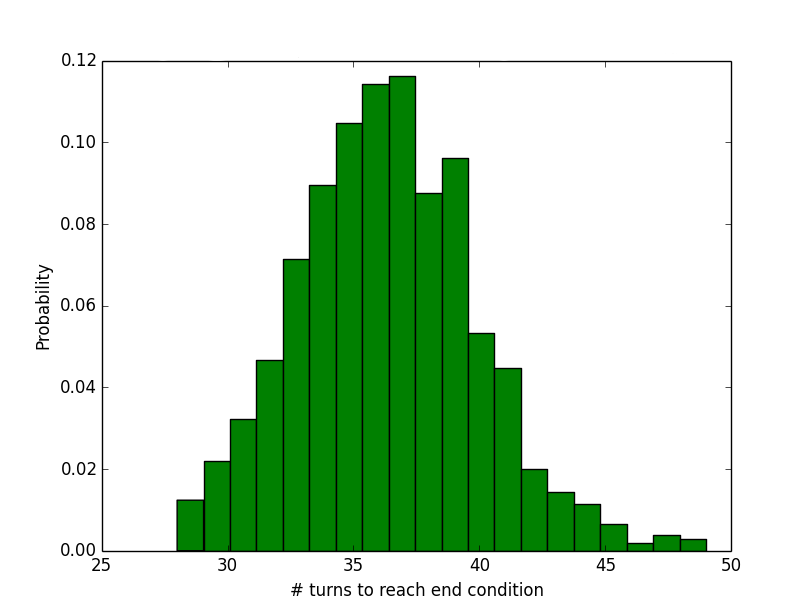
\includegraphics[width=.95\columnwidth]{../pres/village-chancellor-turn-dist.png}
\caption{\label{fig:turn-dist} Probability distribution over number of turns
in a 2-player game of Dominion.
Both players play a greedy strategy with model
parameters of $X = \textrm{Village}$, $Y = \textrm{Chancellor}$, and
$p_0 = 0.5$. See Appendix \ref{app:dominion-card} for a complete description
of the semantics behind these cards and why this pair of cards is interesting
for the game Dominion.
This distributions is unconditioned, therefore only requiring sampling directly
from the model (no inference).
}\end{figure}



